\begin{definition}
    Macierz o wymiarach $m \times n$ i elementach ze zbioru $K$ to odwzorowanie
    \[ \{1, 2, \ldots, m\} \times \{1,2,\ldots,n\} \ni (i, j) \lthen a_{ij} \in K, \]
    które reprezentujemy w następujący sposób:
    \[ \begin{bNiceMatrix}
        a_{11} & a_{12} & \Cdots & a_{1n} \\
        a_{21} & a_{22} & \Cdots & a_{2n} \\
        \Vdots & \Vdots & \Ddots & \Vdots \\
        a_{m1} & a_{m2} & \Cdots & a_{mn}
    \end{bNiceMatrix}. \]
\end{definition}

\begin{definition}
    Macierz transponowana do macierzy $A = [a_{ij}]_{m \times n}$ to macierz
    \[ A^T = [a_{ji}]_{n \times m}. \]
    Jeśli $A = A^T$, to macierz jest \vocab{symetryczna}.
\end{definition}

\vocab{Macierz zerowa} $\mathbf{0}_{m\times n}$ to taka macierz, że wszystkie jej elementy są zerowe. \vocab{Macierz kwadratowa} to macierz o wymiarach $n \times n$. \vocab{Przekątną główną} macierzy kwadratowej tworzą elementy $a_{ii}$.

\begin{definition}
    Macierz diagonalna to macierz kwadratowa, w której wszystkie elementy poza jej główną przekątną są zerowe.
\end{definition}

\begin{definition}
    Macierz jednostkowa to macierz kwadratowa, w której wszystkie elementy na głównej przekątnej są jedynkami. Oznaczamy ją często $I_n$, gdzie $n \times n$ to wymiary tej macierzy.
\end{definition}

\begin{definition}
    Macierz jest trójkątna górna/dolna, jeśli wszystkie elementy poniżej/powyżej głównej przekątnej są równe $0$.
\end{definition}

\subsection{Działania na macierzach}
Zdefiniowane są pewne działania na macierzach:

\paragraph{Suma macierzy} dla macierzy $A = [a_{ij}]_{m \times n}$ i $B = [b_{ij}]_{m \times n}$ tych samych wymiarach:
    \[ A + B = [a_{ij} + b_{ij}]_{m \times n}, \]
\paragraph{Mnożenie przez skalar} dla macierzy $A = [a_{ij}]_{m \times n}$:
    \[ \alpha A = [\alpha a_{ij}]_{m \times n}, \]
\paragraph{Mnożenie macierzy} jeśli liczba kolumn macierzy $A = [a_{ij}]_{m \times p}$ jest równa liczbie wierszy macierzy $B = [a_{ij}]_{p \times n}$, to
    \[ A \cdot B = [c_{ij}]_{m \times n}, \qquad c_{ij} = \sum_{k=1}^p a_{ik}b_{kj}. \]

\begin{figure}[h]
    \centering
    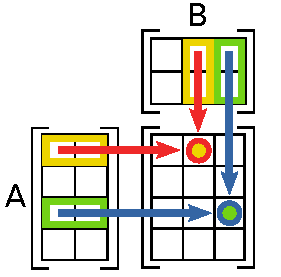
\includegraphics[width=0.3\textwidth]{matrix_multiplication.pdf}
    \caption{Mnożenie macierzy, źródło: Wikipedia.}
\end{figure}

\begin{remark}
    Mnożenie macierzy nie jest przemienne, jest za to łączne i obustronnie rozdzielne względem dodawania.
\end{remark}

\begin{fact}
    Zbiór $M_{m \times n}(\KK)$ macierzy o wymiarach $m \times n$ i elementach z ciała przemiennego $\KK$, $|\KK| \geq 2$ tworzy przestrzeń wektorową nad ciałem $\KK$.
\end{fact}

\begin{fact}
    Elementem neutralnym mnożenia macierzy kwadratowych jest macierz jednostkowa\footnote{jeśli macierz $A_{m\times n}$ nie jest kwadratowa, to również zachodzi $I'M = M$ oraz $M = I''M$ dla pewnych macierzy jednostkowych $I', I''$, lecz $I' \neq I''$ (są różnych wymiarów).}.
\end{fact}

\begin{fact}
    Zachodzi równość
    \[ (AB)^T = B^T A^T. \]
\end{fact}